\section{Method}

In this chapter, the methodologies used for the project are presented. This includes the research methodology, the project methodology, which methods and tools that were used to answer the research question and the technical methodology.

The methodology gives a clearer understanding of how the project was conducted and why the different parts of the project were included.

\subsection{Research methodology}
\label{section:research_methodology}

The research questions for the project were as follows.

\begin{itemize}
    \item Do users notice a difference between progressive web applications and native apps, and does the difference affect the user experience?
    \item Can a model accurately decide whether a PWA, a React Native application or a native application is most favourable?
\end{itemize}

The first question, regarding the user experience, was divided into two sub-tasks:

\begin{itemize}
    \item {Understand how the choice of tool affects user experience (UX)}.
A usability study was performed to understand what affect on UX using different development tools has. 
    \item {Understand how users find mobile applications}.
This sub-task was performed by sending out a market research survey.
\end{itemize}

The second question was divided into two sub-tasks: 

\begin{itemize}
    \item {Understand the limitations of Development tools}.
A literature study and discussions with consultants at Slagkryssaren AB were performed to gather data on the limitations of the development tools.
    \item {Understand the factors involved in choosing a development tool}.
\end{itemize}

The factors for choosing a development tool were explored in discussions with consultants at Slagkryssaren AB. 

The study followed the four-step method of Pólya. This method was chosen since it divided the main problem into smaller, more perspicuous problems. This method allowed for an iterative work process, which would produce deliverable products that could have been improved on in increments. The model contains four steps: Understand the problem, Devise a plan, Implement the plan, and Evaluate and control \cite{PolyaPDF}.
The four-step method and its parts can be seen in figure \ref{fig:project-polya}.

\begin{figure}[ht]
    \centering 
    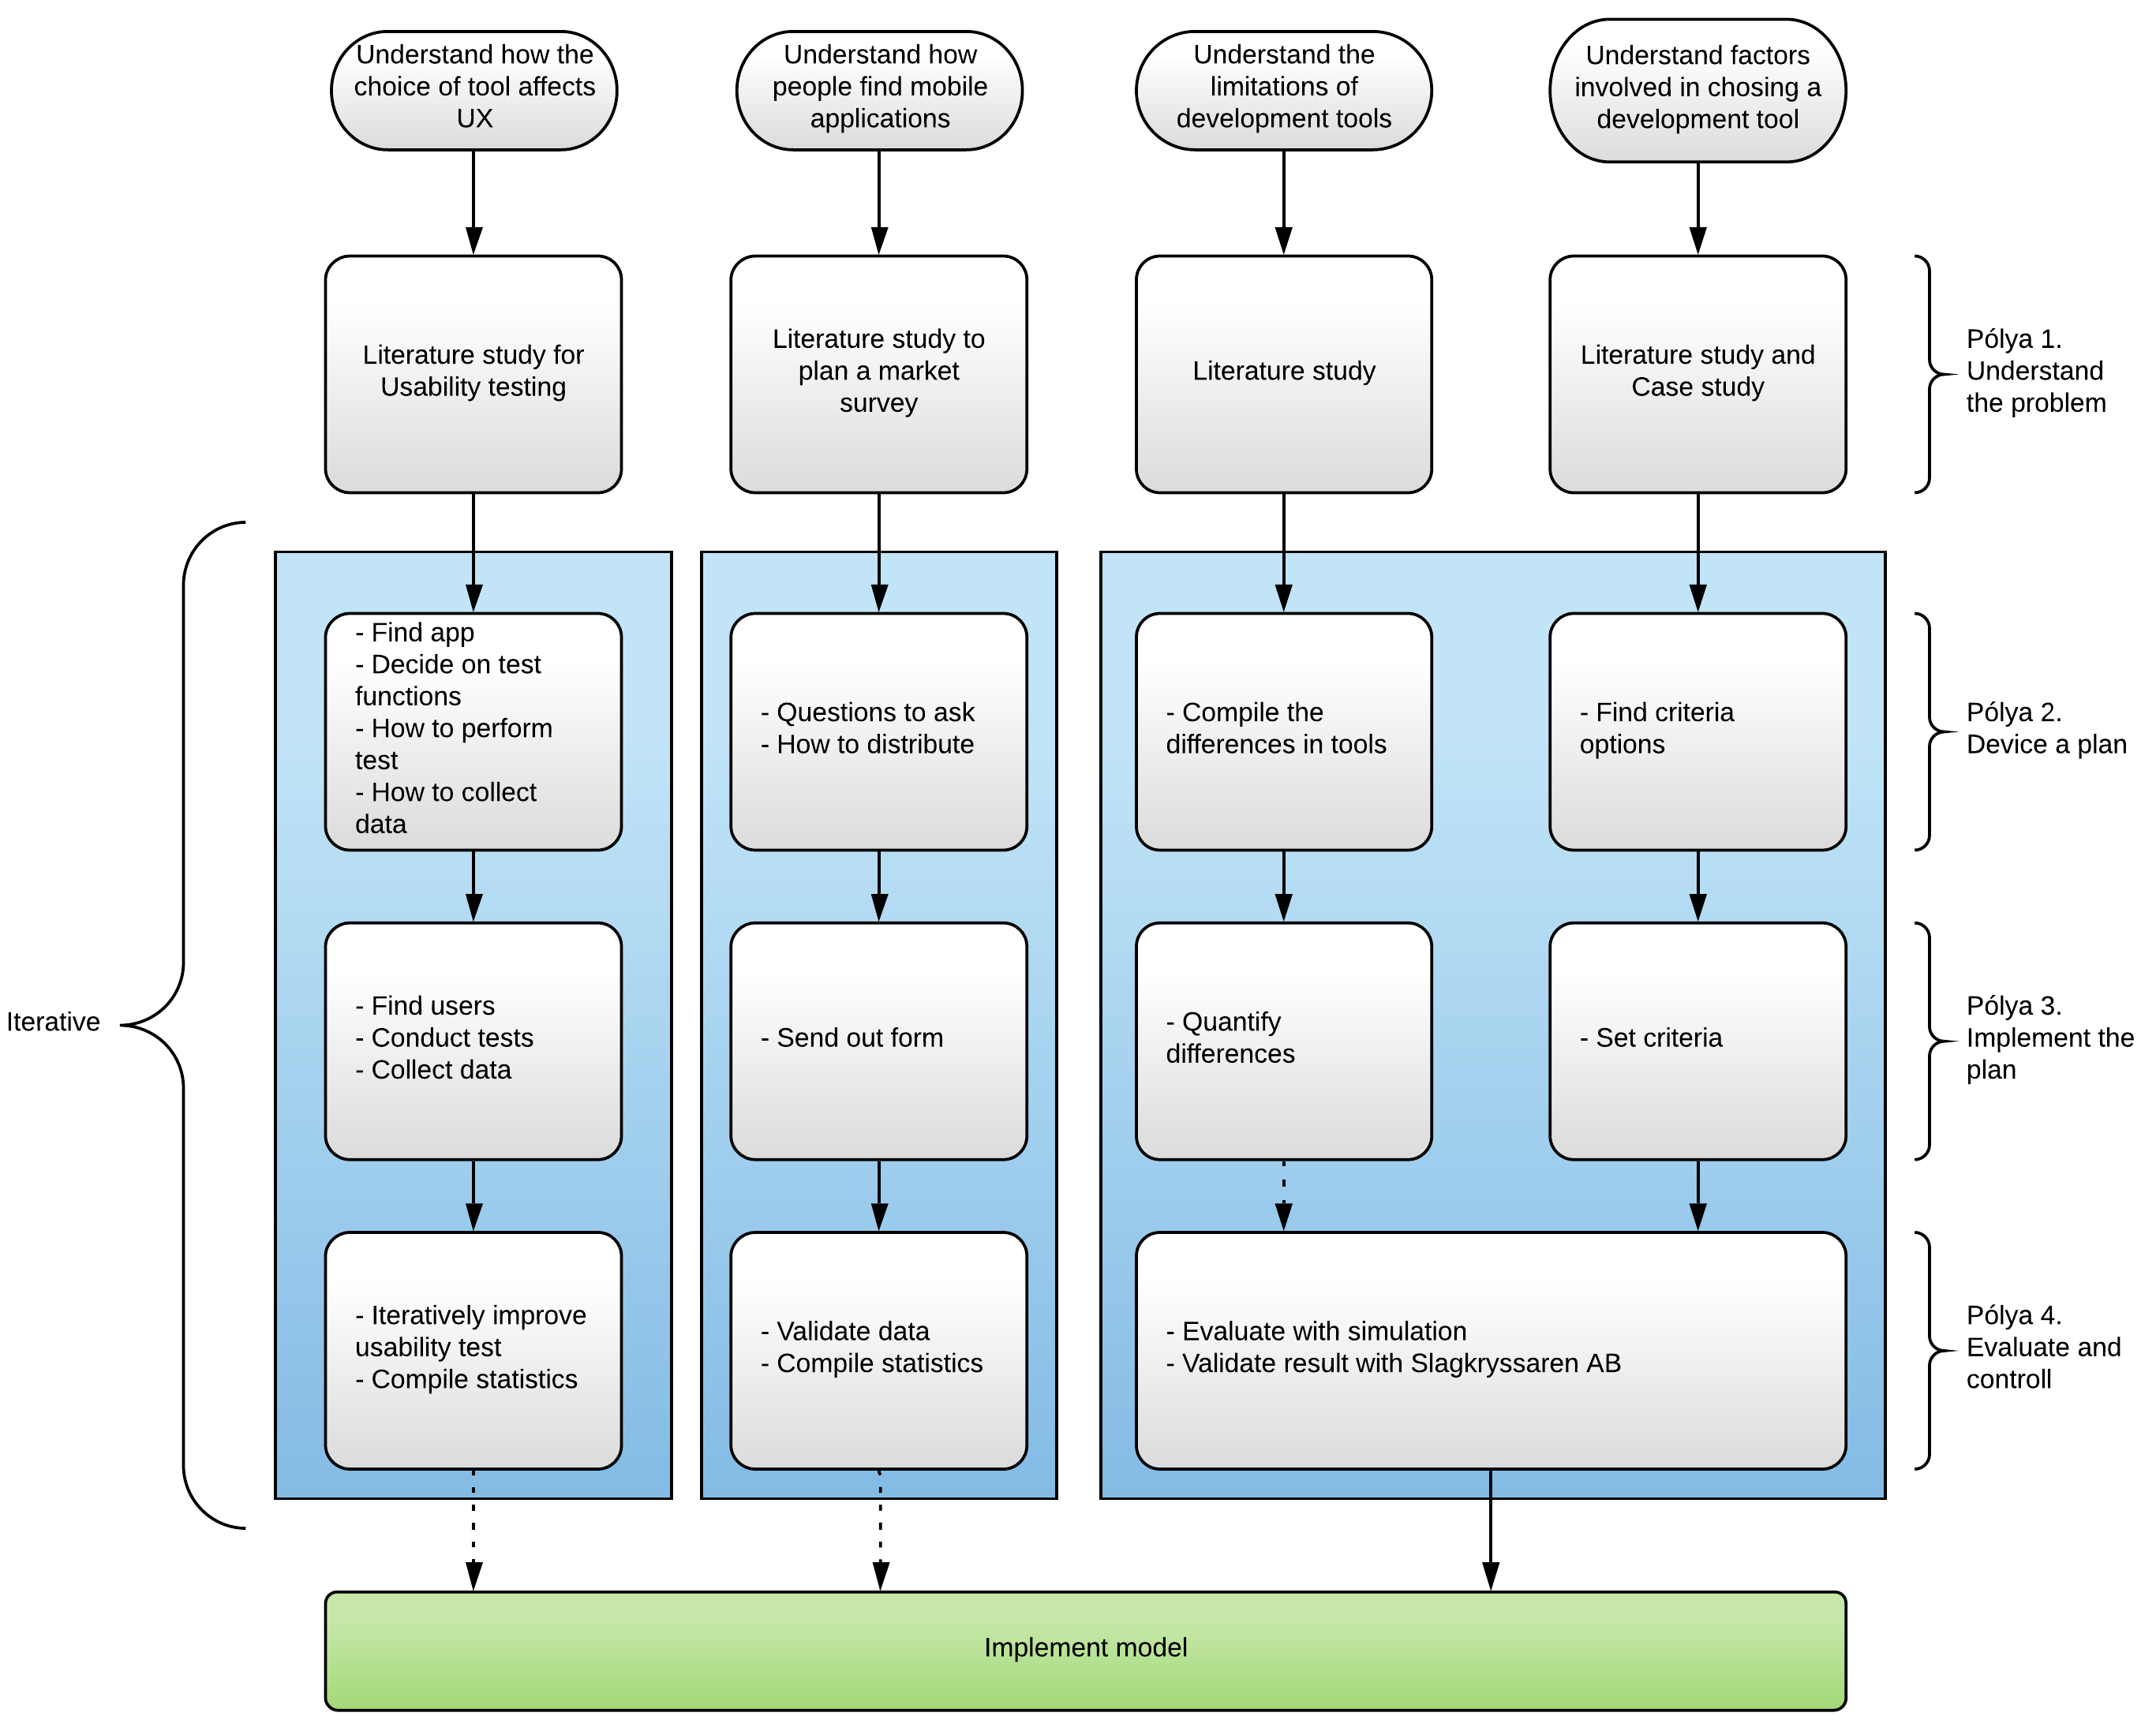
\includegraphics[width=1\textwidth]{img/polya2.png}
    \hfill
    \caption{\textit{Implementation of Pólya's four-step method.}}
        \label{fig:project-polya}
\end{figure}

\subsection{Project methodology}

The project methodology is a process which guides the project from a plan to a finished product. Resource management, cost efficiency and prioritization are some of the factors to consider when entering a new project, and following a well-defined project method would increase the chances of producing deliverable results with the resources available. 

\subsubsection{The project triangle}

The project triangle, shown in figure \ref{fig:project_triangle}, describes how the quality of the project correlates with the time, cost and scope  \cite{TheProjectTriangle}. The cost and time of this project were predetermined, so the only mobile variable was the scope. This means that the scope of the project could have been extended or cut as needed. This could have been applied to the usability tests, as more or fewer tests could have been conducted depending on the time left. Extending the scope could, for example, mean introducing more technologies into the model. The scope could also have been extended, improving the quality, if more tests had been conducted.

\begin{figure}[ht]
    \centering 
    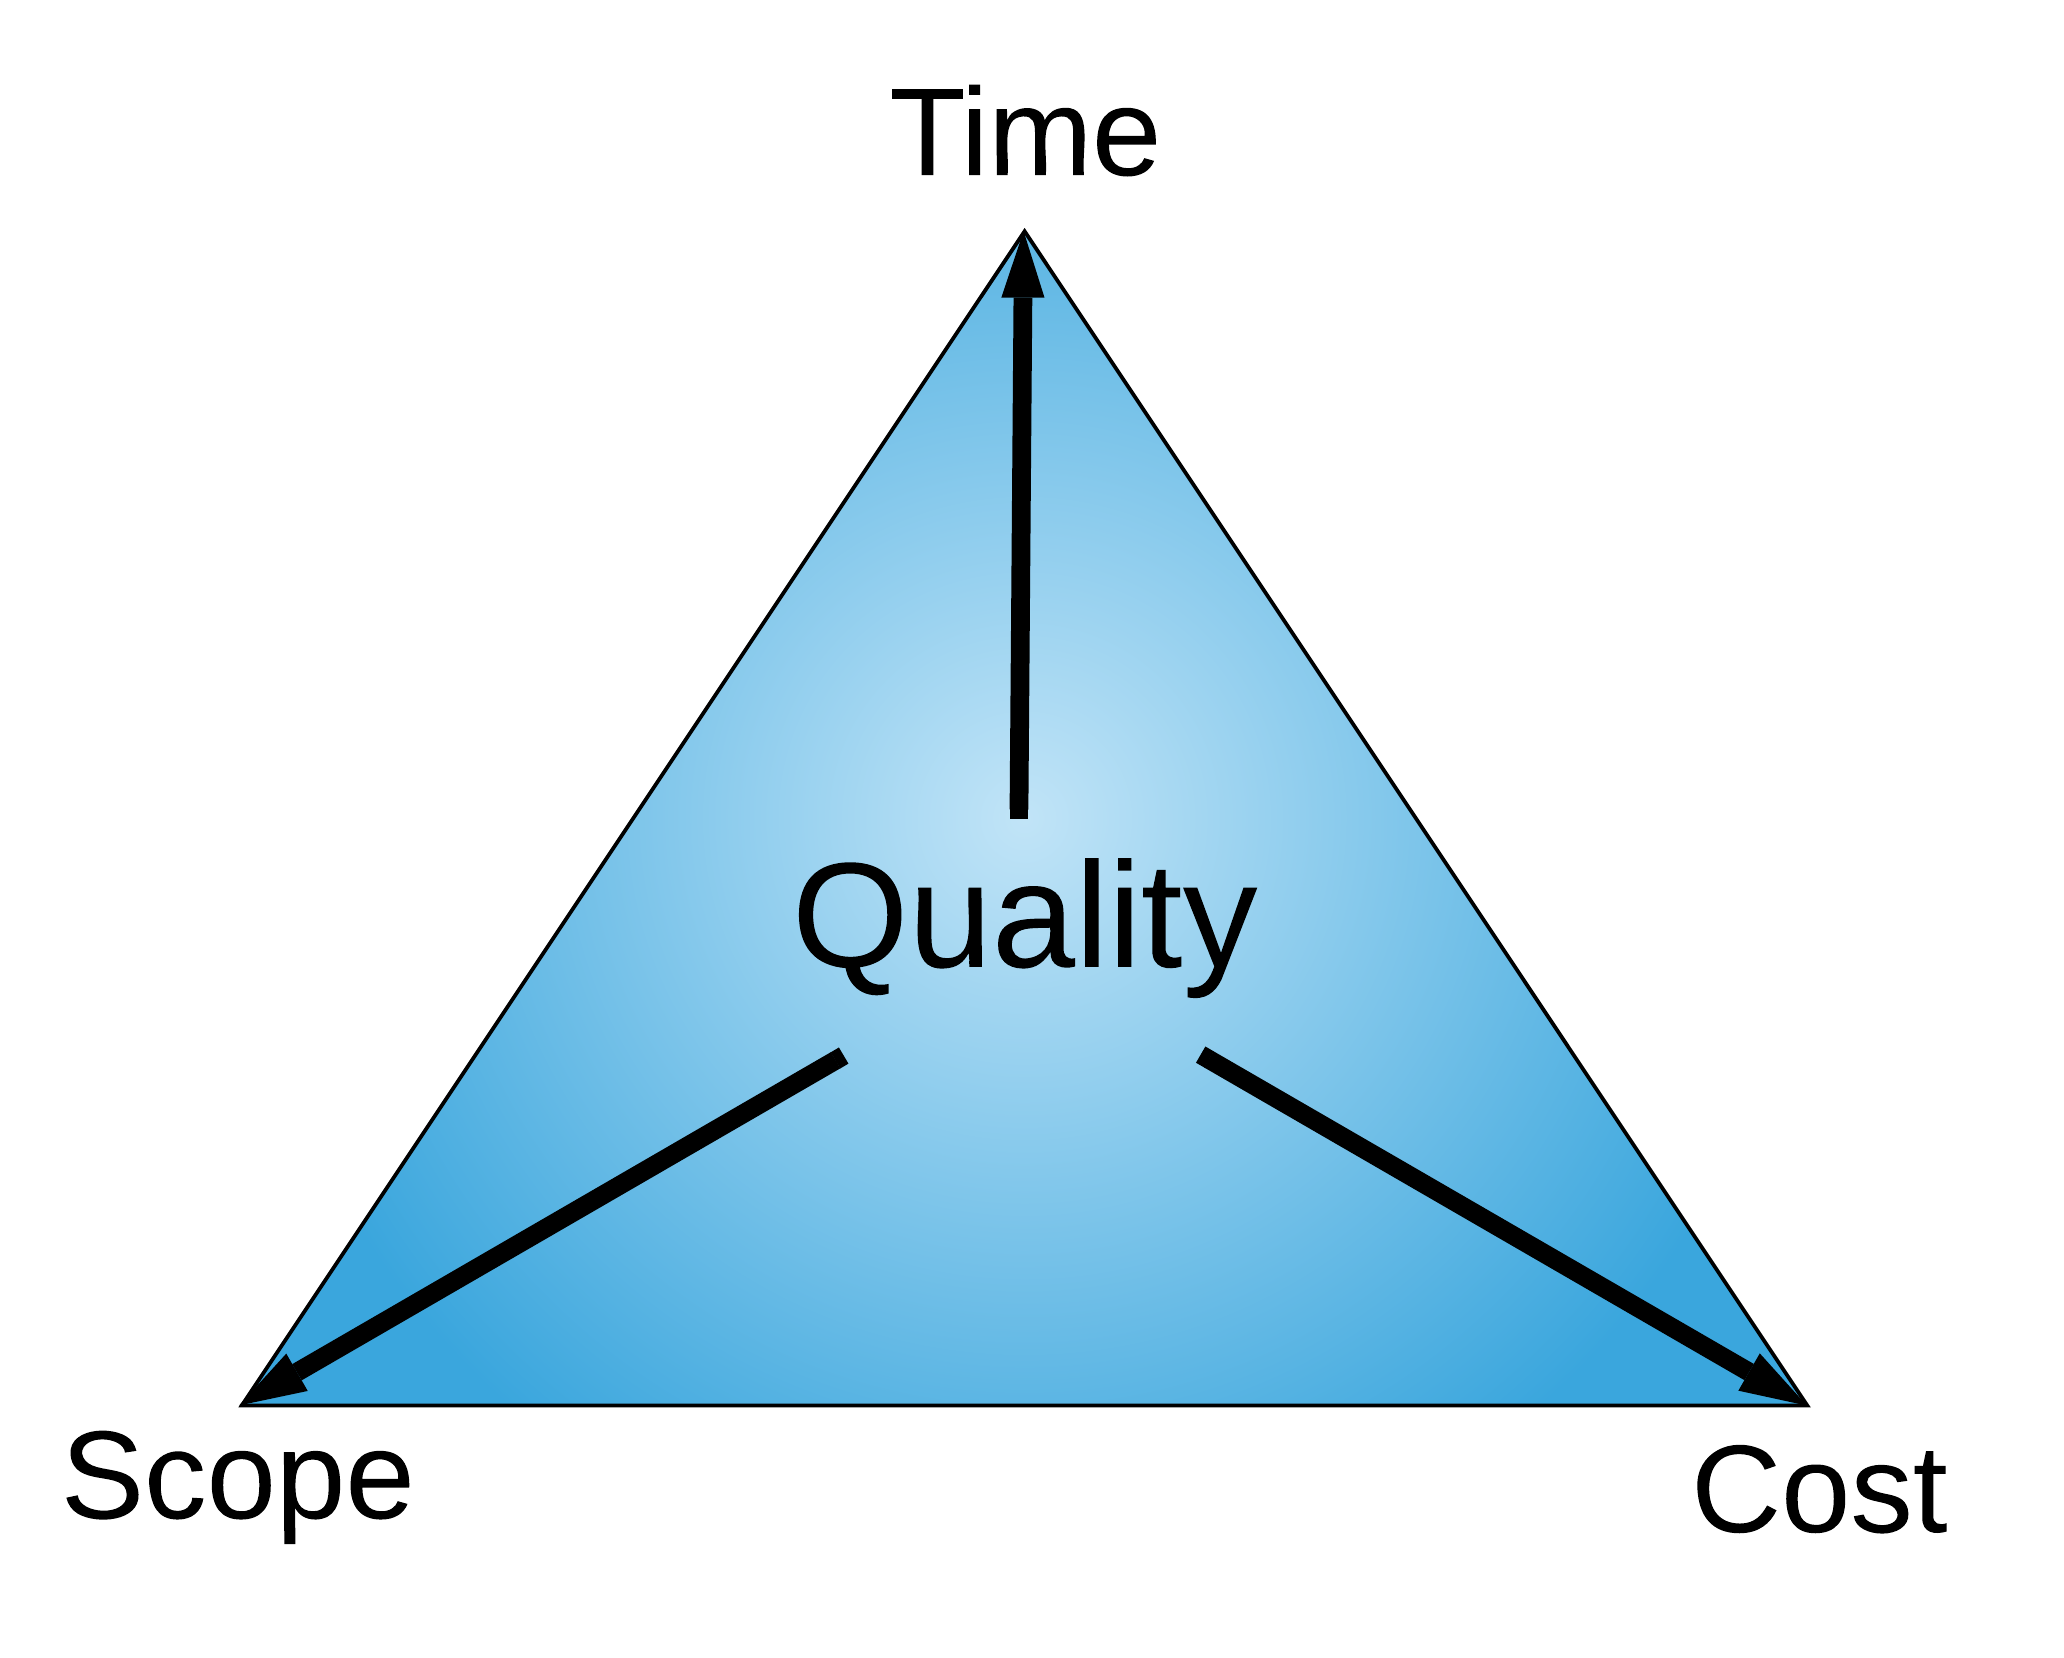
\includegraphics[width=0.6\textwidth]{img/project_triangle.png}
    \hfill
    \caption{\textit{The project triangle}}
    \label{fig:project_triangle}
\end{figure}

\subsubsection{MoSCoW}

MoSCoW is a method used to prioritize during project management \cite{MoSCoWforUX}. The term MoSCoW is an acronym for the four prioritization categories: Must have, Should have, Could have and Won’t have. The MoSCoW was chosen as a prioritization method for this project due to its ability to fraction the project into a core assignment and possible improvements. 
The MoSCoW for this project can be seen in figure  \ref{fig:MoSCoW}.

\begin{figure}[ht]
    \centering 
    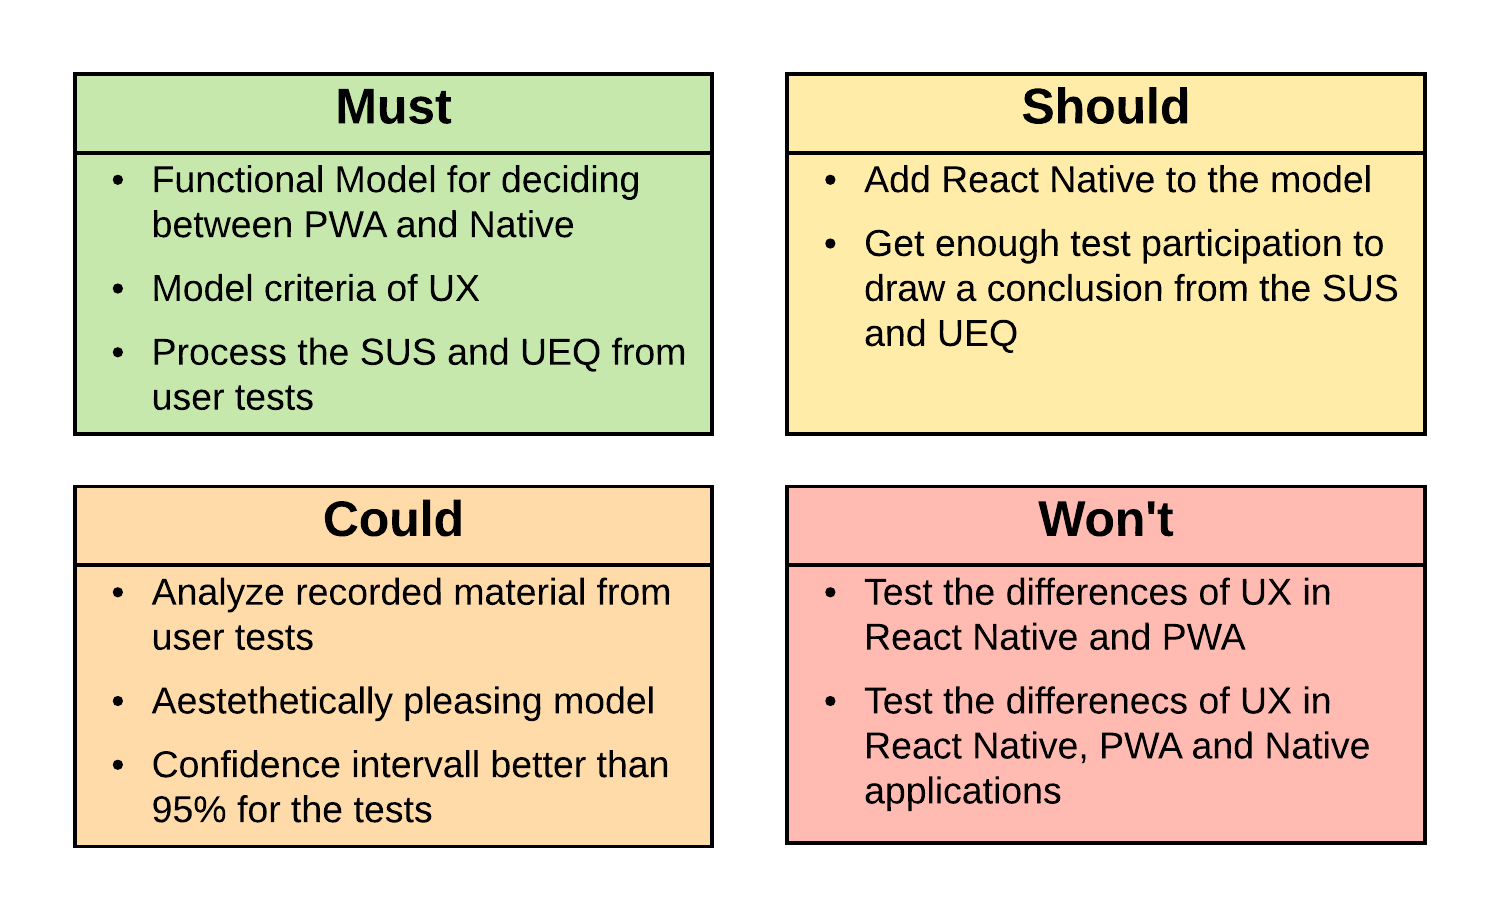
\includegraphics[width=0.9\textwidth]{img/moscow.png}
    \hfill
    \caption{\textit{MoSCoW chart of this project}}
    \label{fig:MoSCoW}
\end{figure}

\subsubsection{Connecting the dots}

With the research and project methodology explained and established it was easier to get hold of the overall picture of this study. The scope and iterations were limited by the time and the cost, two factors which this study could not affect. When the tasks of the MoSCoW category "Must" had been fulfilled, depending on how much time was left, more tasks from the categories "Should" and "Could" could have been added to the project.

\subsection{Literature Study}

To understand and explore the differences between the different types of mobile applications, extensive research had to be made. Mobile applications that use more of a hybrid approach, such as PWA or React Native, tend to follow trends. This means that if the technology does not get enough attention it might go extinct. This was at the time of writing happening to many JavaScript frameworks such as Angular, according to consultants at Slagkryssaren AB. The information available on this subject was both opinion- and research-based.

For the MCDM, the design practices and evaluation processes were investigated. 
To conduct usability testing, it was a requirement that these tests should follow typical practices currently in use. This includes how to design, conduct and validate usability tests.
Typical places where information was gathered were:

\begin{itemize}
    \item Blogs, forums and similar websites
    \item Research articles and technical literature 
    \item Opinions from developers and experts within interaction design
\end{itemize}

\subsection{Case study}

Since the model was to be used by Slagkryssaren AB, the development of the model was done in close co-operation with the company’s consultants. These consultants have extensive experience in the field of developing applications and choosing application development tools. This inductive approach was more suitable than a deductive one, as there was no decidedly right or wrong conclusion when choosing an application development tool.

Conduction of the case study was done by discussion with the consultants at Slagkryssaren AB. These discussion meetings were to be unstructured in an attempt to get richer, more qualitative data. A combination of planned and improvised discussions were held to answer questions emerging during the progression of the study. The meetings were held approximately once a week, and lasted around 40 minutes each.

\subsection{Mobile application discovery survey}

The survey was conducted to explore two hypotheses which emerged during the discussions with Slagkryssaren AB, one of them being that people tend to find information about applications mostly on the platforms application store, rather than using web searches. The other hypothesis was that Android users tend to look for information about applications through web searches, while iPhone users tend to go to the App Store first. This hypothesis was based mainly on the fact that smartphones running Android usually have a Google search bar pre-installed on the home screen. It would therefore be easier for them to just tap the search bar to find information, rather than opening the App store application which one has to do on iOS devices. These hypothesis were explored to understand the consequences of releasing an application which can not be found on the platform’s app store, which is the case for PWAs. 

\subsection{Usability testing}

To see the differences in user experience, usability tests were conducted. Usability testing was chosen as a method for measuring UX due to its relative simplicity and time efficiency.

During the tests, PWA and native applications had the main focus. React Native and PWA both use JavaScript but React Native can access native user interface components, meaning it is like a mixture of both types. To be able to perform the usability tests with all tree techniques we would have needed a similar application developed with all methods, something that was not available at that moment, and outside of the scope of this study to develop. 

To measure the differences in quality, usability, attractiveness and other UX-related criteria, validation of the tests was done using surveys. Several measuring methods for this exist, such as the System Usability Scale (SUS), the Usability Experience Questionnaire (UEQ), Net Promoter Score and the Standardized User Experience Percentile Rank Questionnaire. These surveys are popular for measuring how good the different applications are in certain criteria \cite{Rauschenberger2013, Kortum2014}. The surveys can only receive quantifiable data.  A better overview of the process of the tests is shown in figure \ref{fig:usability_test_process}.

The users tested two versions of the same application on the same platform they normally used. One of the application versions was a PWA and the other a native application.

The subject got a list of six tasks to perform on the application, and after using each version of the application the subjects filled in a UEQ and a SUS form. The results from these SUSs and UEQs formed the base for the quantitative data from the usability tests. During the tests, the moderator encouraged the subject to keep talking by asking questions about what the subject was doing. To fully understand the test subject’s experience, it was useful to have them think out loud. This means the subject says out loud what they are thinking and trying to do while testing the application, giving the researcher an insight into what the subject has troubles with and misunderstands in the product. Thinking out loud gave qualitative data from the users \cite{Nielsen2012}.

After both applications had been tested, the subject was asked more in-depth questions about their experience of the applications and their thoughts and feeling. This gave richer, more nuanced comparisons between the different applications, and qualitative information which could later be processed to further define how the criterion for UX should be scored in the model.

The recorded material from the tests was analyzed. The subjects’ feelings about the applications were interpreted through their spoken words, their facial expressions and verbal cues. This data was then quantified by processing the recorded material and transcriptions, in search of patterns in the subjects’ behaviour.

The results from the UEQ and SUS were plotted and compared between the two application. With this data, a confidence interval could be calculated and compared to the preferred confidence level. This result formed the basis for the criterion of UX.

\begin{figure}[ht]
    \centering 
    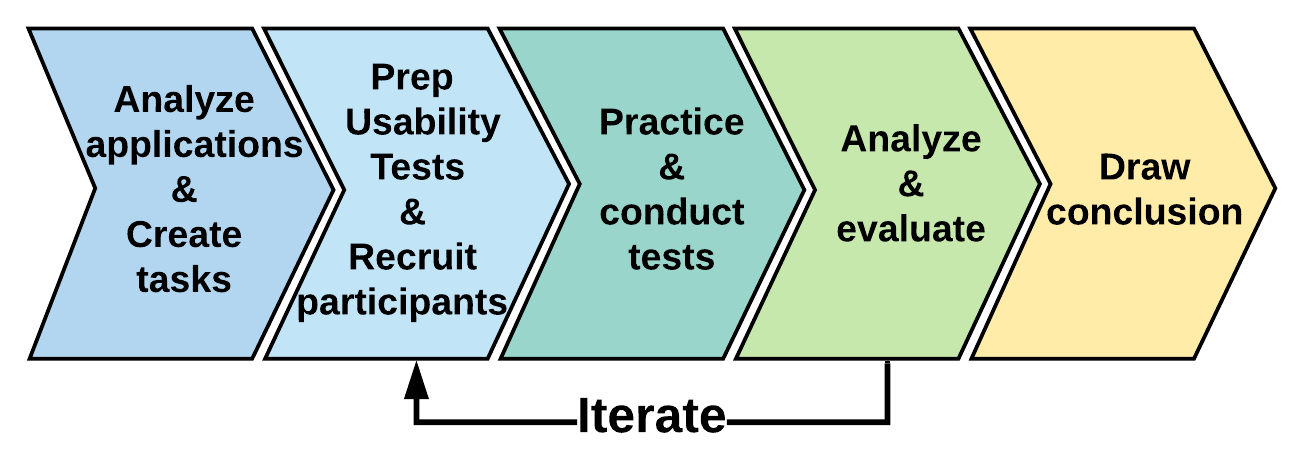
\includegraphics[width=0.9\textwidth]{img/usability_test_process.png}
    \hfill
    \caption{\textit{Process of performing a usability test}}
    \label{fig:usability_test_process}
\end{figure}

\subsection{Multi-Criteria Decision-Method}

To build a model which took usability into account, the comparative usability test was conducted. This inductive approach would produce qualitative data. The different solutions tested in a comparative usability test could be tested either separately on the different test subject, or together on the same subjects. In this study, both solutions were tested on all test subjects. A drawback with this method is that there could emerge a pattern that the user would like a particular version if they are tested in the same order \cite{Ross2017}. To counteract this effect the subjects tested the applications in varying order so that the bias would have the same impact in both directions, hopefully cancelling out in the end. This was done since the scope of the study was comparatively small, meaning the benefit of more test subjects was vital.

To make the results as comparable as possible, we chose to have all the test subjects perform the same set of tasks. The tests were conducted on the same OS that the test subject normally used, to minimize confusion due to an unknown platform  \cite{Schultz2006}. 
For the model, it was also relevant to include application exploration as a criterion. To acquire quantitative data for the finding and downloading habits of the population, a cross-sectional survey was conducted. This gave data from a more diverse population than is possible from qualitative methods, such as interviews, in the span of the study. 

The model itself was based on the MCDM method. The MCDM uses a mathematical function to calculate the best alternative when faced with a decision involving many different criteria. The decision-makers decide which criteria are important and rank them. The possible alternatives are then scored on each criterion. The alternative with the highest score is then the best alternative for that decision-makers ranking.

Several MCDM methods could have been applied to this study. WSM was chosen due to its simplicity of calculation. Since the WSM demands the data to be quantifiable, all qualitative data gathered was translated into quantitative data. 
Mobile application discovery was researched with an online survey, producing quantified data. 

For the tests, quantification was done with surveys and questionnaires where test subjects quantified their own experience with the application, in combination with analyzed facial expressions and behaviour from the recordings.

The criteria were based on input from results of our test and survey, scientific articles, software development websites and discussions with consultants at Slagkryssaren AB.

When a set of criteria was decided, scores were given to each alternative development tool in the model. The scores were set based on previous literature study. These scores were presented to the consultants at Slagkryssaren AB and were iteratively improved upon based on their feedback.

When scores were set for the alternatives, the next iterative phase began. 
Use cases were run through the model, and the result was assessed. If the outcome was seen as unreasonable or unlikely to be chosen, the scores and criteria were reassessed. This iterative process was to be repeated until reasonable results are acquired, or until there was no more time to reiterate. 

\subsection{Technical method}

In order for this study to be carried out, there was need to include some tools. Testing different ways of calculating the decision-making model and analyzing the data from the survey, UEQ and SUS was done using \textit{Google sheets}. Gathering the data for the tests and survey was done using \textit{Google forms}. The recording of the usability tests was done using an \textit{Asus} laptop and a \textit{GoPro Hero 4 Session}. All the gathered data and other media were stored on \textit{Google drive}. The devices that were used for the tests are \textit{Apple iPhone 11 Pro} and \textit{Oneplus 5}. The model was implemented using the javascript framework  \textit{Vue.js}, and stored on \textit{GitHub}.  